\chapter{सममिति और बिंदु समूह}\label{ch:b3:point-groups}

किसी हिमकण को साठ अंश घुमाइए और कुछ नहीं बदलता; बेंज़ीन अणु को उतने ही कोण से
घुमाइए, और उसके छह कार्बन और छह हाइड्रोजन ठीक एक-दूसरे के स्थानों पर आ
जाते हैं। किसी अणु की सममिति किसी भी परिकलन से पहले उसके कई गुणधर्म तय कर देती
है: क्या उसका द्विध्रुव आघूर्ण हो सकता है, क्या वह दो दर्पण-प्रतिबिंब रूपों में
रह सकता है, उसके कौन-से कंपन अवरक्त प्रकाश अवशोषित करते हैं, कौन-से कक्षक मिश्रित
हो सकते हैं। इसका उपयोग करने के लिए रसायनज्ञों ने गणित से समूहों की भाषा उधार ली।
यह अध्याय किसी अणु की \omterm{def:b3:point-groups:operation}{सममिति संक्रियाओं} को परिभाषित करता है, उन्हें उसके \omterm{def:b3:point-groups:point-group}{बिंदु
समूह} में एकत्र करता है, वह समूह ज्ञात करने की एक प्रक्रिया देता है, ध्रुवता और
किरैलता पर दो प्रमेय सिद्ध करता है, और उन \omterm{def:b3:point-groups:irrep}{अभिलक्षण सारणियों} का परिचय देता है जिन पर
\cref{ch:b3:group-theory-applied} आगे निर्माण करता है।

\begin{recall}
प्रथम वर्ष के खंड ने VSEPR मॉडल से आण्विक आकृतियों की भविष्यवाणी की,
ध्रुवीय अणु के द्विध्रुव आघूर्ण को परिभाषित किया, और किरैलता को परिभाषित किया: किरैल
अणु को उसके दर्पण-प्रतिबिंब पर अध्यारोपित नहीं किया जा सकता। द्वितीय वर्ष के खंड ने
\ce{H2O} और \ce{NH3} के अणुखंड कक्षक बनाने के लिए सममिति का शब्दों में उपयोग किया।
\end{recall}

\begin{omfigure}
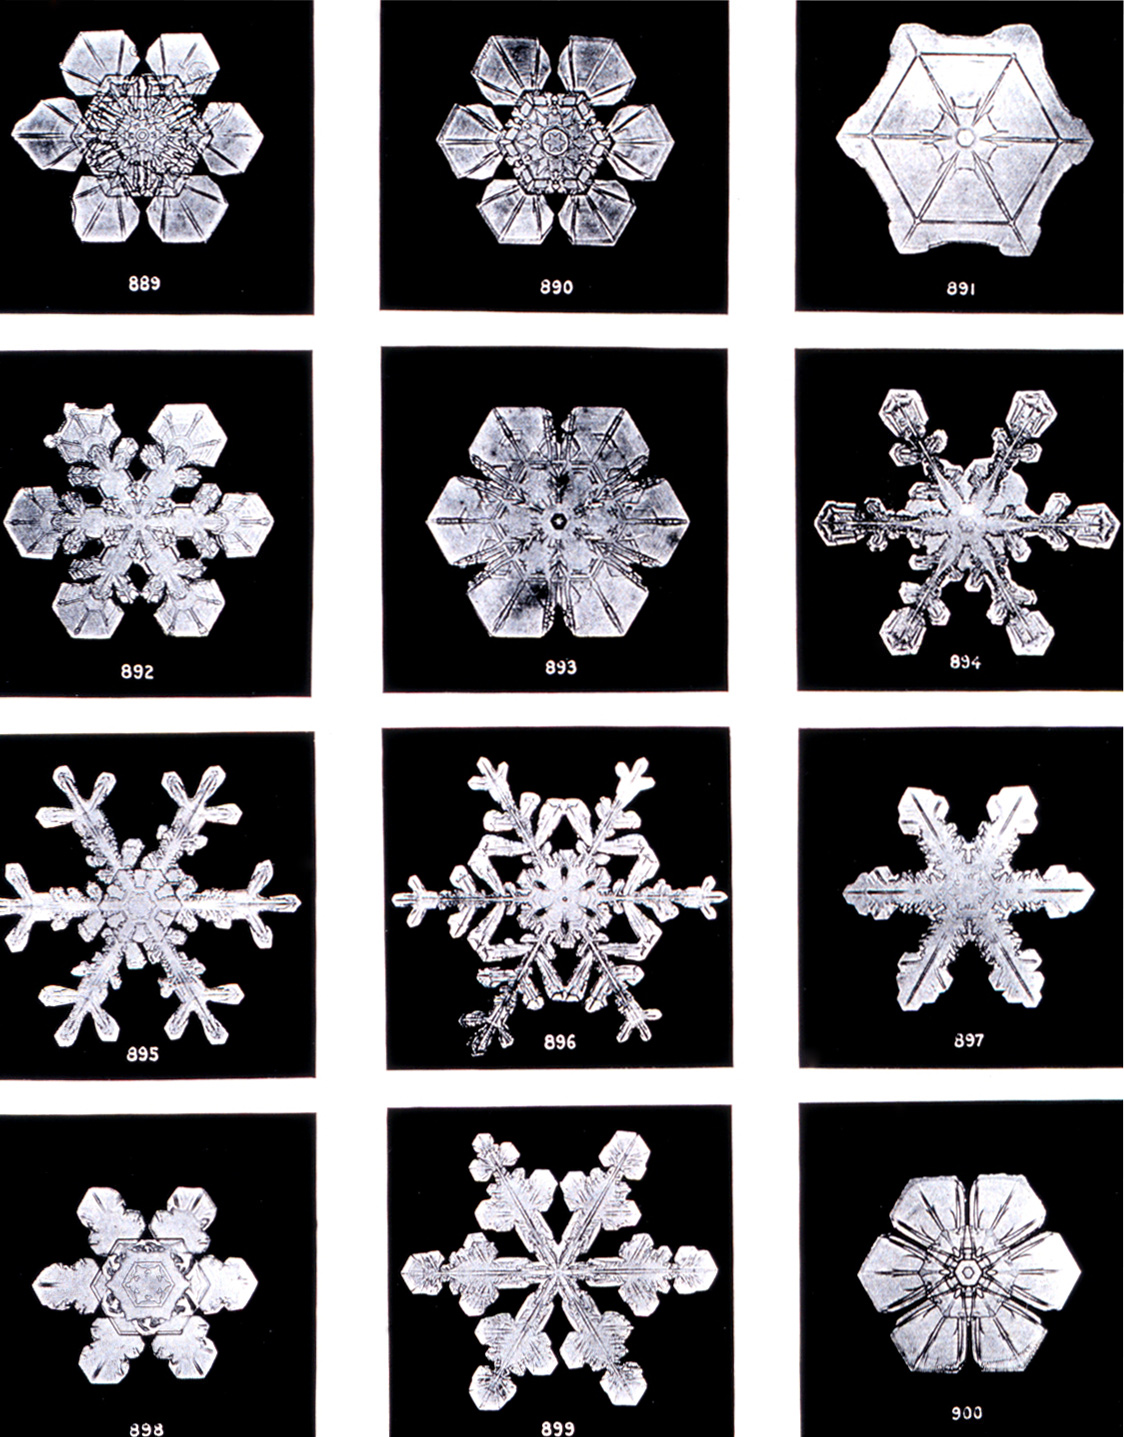
\includegraphics[width=0.4\linewidth]{images/book4/bentley-snowflakes.jpg}\hspace{1em}%
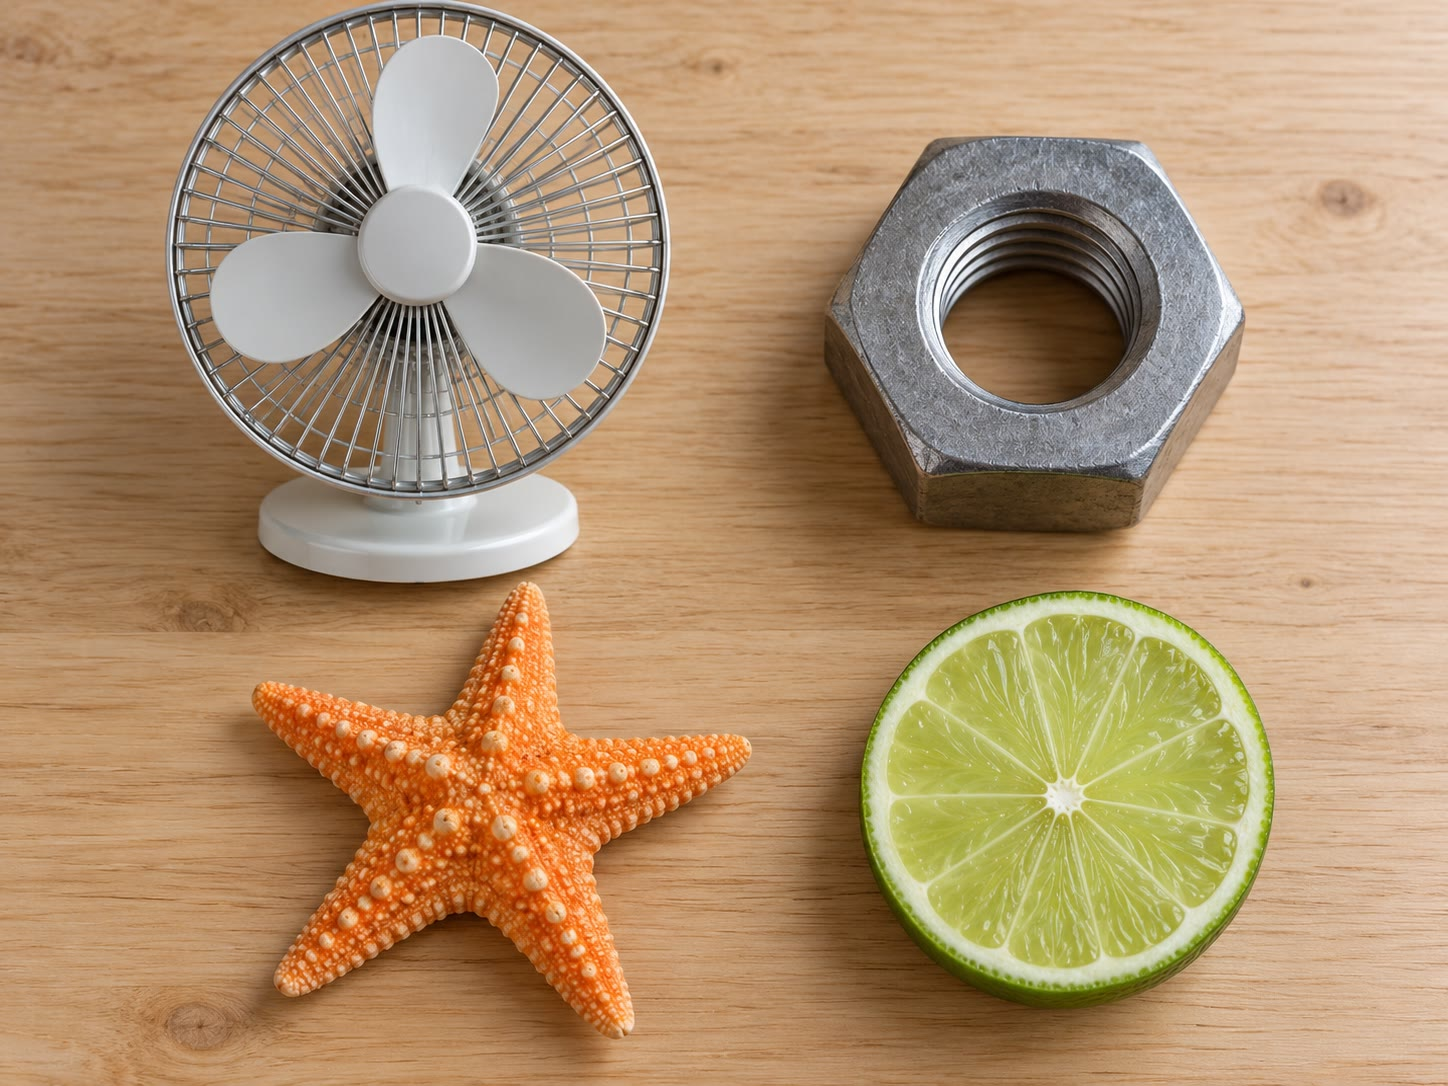
\includegraphics[width=0.48\linewidth]{images/book4/ai/b3-04-symmetric-objects.jpg}

{\small बाएँ: लगभग 1902 में विल्सन बेंटली द्वारा छायाचित्रित हिम-क्रिस्टल,
हर एक षड्गुण सममिति वाला। दाएँ: त्रिगुण, षड्गुण और पंचगुण घूर्णन सममिति वाली
दैनिक जीवन की वस्तुएँ।}
\end{omfigure}

\section{सममिति संक्रियाएँ और सममिति तत्व}

\begin{definition}[सममिति संक्रिया, सममिति तत्व]\label{def:b3:point-groups:operation}
\emph{सममिति संक्रिया}\index{सममिति संक्रिया} ऐसी गति या
परावर्तन है जो किसी अणु को ऐसे विन्यास में छोड़ता है जो मूल से अविभेद्य हो
(हर परमाणु ऐसी स्थिति पर, जिस पर पहले उसी प्रकार का परमाणु था)।
\emph{सममिति तत्व}\index{सममिति तत्व} वह ज्यामितीय
वस्तु है --- एक बिंदु, एक रेखा, एक तल --- जिसके सापेक्ष संक्रिया
की जाती है।
\end{definition}

हर अणु में तत्समक संक्रिया $E$ होती है, जो कुछ नहीं करती। बाकी
संक्रियाएँ चार प्रकार की होती हैं।

\begin{definition}[उचित घूर्णन अक्ष, मुख्य अक्ष]\label{def:b3:point-groups:rotation}
\emph{उचित घूर्णन अक्ष}\index{उचित घूर्णन अक्ष} $C_n$ वह रेखा है
जिसके परितः $2\pi/n$ का घूर्णन एक \omterm{def:b3:point-groups:operation}{सममिति संक्रिया} है, जिसे भी
$C_n$ लिखा जाता है; इसकी घातें $C_n^k$, $2\pi k/n$ के घूर्णन हैं, और $C_n^n = E$।
उच्चतम $n$ वाला अक्ष \emph{मुख्य अक्ष}\index{मुख्य अक्ष} है, जिसे
$z$ लिया जाता है।
\end{definition}

\begin{definition}[दर्पण तल]\label{def:b3:point-groups:mirror}
\emph{दर्पण तल}\index{दर्पण तल} $\sigma$ वह तल है जिसमें
परावर्तन एक \omterm{def:b3:point-groups:operation}{सममिति संक्रिया} है; $\sigma^2 = E$। कोई दर्पण तल
\emph{ऊर्ध्वाधर दर्पण तल}\index{ऊर्ध्वाधर दर्पण तल} $\sigma_v$ है यदि उसमें
\omterm{def:b3:point-groups:rotation}{मुख्य अक्ष} समाहित हो, \emph{क्षैतिज दर्पण
तल}\index{क्षैतिज दर्पण तल} $\sigma_h$ यदि वह उसके लंबवत
हो, और \emph{द्वितल दर्पण तल}\index{द्वितल दर्पण तल}
$\sigma_d$ यदि उसमें \omterm{def:b3:point-groups:rotation}{मुख्य अक्ष} समाहित हो और वह उसके लंबवत दो $C_2$ अक्षों के
बीच के कोण को समद्विभाजित करे।
\end{definition}

\begin{definition}[प्रतिलोमन केंद्र]\label{def:b3:point-groups:inversion}
\emph{प्रतिलोमन केंद्र}\index{प्रतिलोमन केंद्र} $i$ वह बिंदु है
जिसके सापेक्ष प्रतिलोमन, $(x, y, z) \mapsto (-x, -y, -z)$, एक \omterm{def:b3:point-groups:operation}{सममिति
संक्रिया} है।
\end{definition}

\begin{definition}[अनुचित घूर्णन अक्ष]\label{def:b3:point-groups:improper}
\emph{अनुचित घूर्णन अक्ष}\index{अनुचित घूर्णन अक्ष} $S_n$ वह
रेखा है जिसके परितः $2\pi/n$ का घूर्णन, और उसके बाद उसके लंबवत
तल में परावर्तन, एक \omterm{def:b3:point-groups:operation}{सममिति संक्रिया} है। $S_1 = \sigma$ और $S_2 = i$।
\end{definition}

\begin{example}[चार अणुओं के तत्व]\label{ex:b3:point-groups:elements}
\ce{H2O}: $E$, H--O--H कोण को समद्विभाजित करने वाला एक $C_2$ अक्ष, और दो ऊर्ध्वाधर
तल, आण्विक तल और उसके लंबवत तल। \ce{NH3}:
$E$, N से होकर एक $C_3$ (संक्रियाएँ $C_3$ और $C_3^2$), और तीन $\sigma_v$, हर एक में
एक N--H आबंध। \ce{BF3}: एक $C_3$, B--F आबंधों के अनुदिश तीन $C_2$,
$\sigma_h$ (आण्विक तल), तीन $\sigma_v$, और एक $S_3$। \ce{CH4}: C--H आबंधों के
अनुदिश चार $C_3$, H--C--H कोणों को समद्विभाजित करने वाले तीन $C_2$, जो
$S_4$ अक्ष भी हैं, और छह $\sigma_d$, हर एक में दो C--H आबंध
(नीचे का चित्र)।
\end{example}

\begin{omfigure}
\begin{tikzpicture}[font=\small]
  % H2O, side view: molecular plane xz (shaded), C2 along z
  \begin{scope}
    \fill[omDef!10] (-1.5,-1.0) -- (1.5,-1.0) -- (1.5,1.2) -- (-1.5,1.2) -- cycle;
    \fill[omThm!12, opacity=0.8] (-0.45,-1.35) -- (0.45,-0.65) -- (0.45,1.55) -- (-0.45,0.85) -- cycle;
    \draw[densely dashed, black!70] (0,-1.4) -- (0,1.7) node[above] {$C_2$};
    \node[aO] (o) at (0,0.5) {};
    \node[aH] (h1) at (-0.95,-0.25) {};
    \node[aH] (h2) at (0.95,-0.25) {};
    \begin{scope}[on background layer]
      \draw[bond] (o.center) -- (h1.center) (o.center) -- (h2.center);
    \end{scope}
    \node[omDef, anchor=north west] at (-1.5,1.2) {$\sigma_v(xz)$};
    \node[omThm, anchor=west] at (0.5,-0.85) {$\sigma_v'(yz)$};
    \node[anchor=north] at (0,-1.6) {\ce{H2O}, $C_{2v}$};
  \end{scope}
  % NH3, top view along C3
  \begin{scope}[xshift=4.0cm]
    \foreach \a in {90,210,330}{\draw[ommirror] (0,0) -- (\a:1.35); \draw[ommirror, black!40] (0,0) -- (\a+180:1.0);}
    \foreach \a in {90,210,330}{\node[aH] at (\a:0.95) {};}
    \node[aN] at (0,0) {};
    \pic at (0,0) {omthreefold};
    \node[anchor=north] at (0,-1.6) {\ce{NH3}, $C_{3v}$ (ऊपर से)};
  \end{scope}
  % BF3, top view; sigma_h = plane of the paper (thick circle)
  \begin{scope}[xshift=8.0cm]
    \draw[ommirror] (0,0) circle (1.3);
    \foreach \a in {90,210,330}{\draw[ommirror] (\a:1.3) -- (\a+180:1.3);}
    \foreach \a in {90,210,330}{\pic[rotate=\a-90] at (\a:1.42) {omtwofold}; \pic[rotate=\a-90] at (\a+180:1.42) {omtwofold};}
    \foreach \a in {90,210,330}{\node[aF] at (\a:0.95) {};}
    \node[aX={pink!70!gray}{5.6mm}] at (0,0) {};
    \pic at (0,0) {omthreefold};
    \node[anchor=north] at (0,-1.6) {\ce{BF3}, $D_{3h}$ (ऊपर से)};
  \end{scope}
\end{tikzpicture}

{\small \omterm{def:b3:point-groups:operation}{सममिति तत्व}। \ce{H2O}: $C_2$ अक्ष (खंडित) और दो \omterm{def:b3:point-groups:mirror}{ऊर्ध्वाधर
दर्पण तल}। \ce{NH3} और \ce{BF3} अपने \omterm{def:b3:point-groups:rotation}{मुख्य अक्ष} के अनुदिश देखे गए (त्रिभुज
चिह्न): मोटी रेखाएँ किनारे से देखे गए \omterm{def:b3:point-groups:mirror}{दर्पण तल} हैं; \ce{BF3} में मोटा
वृत्त \omterm{def:b3:point-groups:mirror}{क्षैतिज दर्पण तल} (पृष्ठ का तल) दर्शाता है और
लेंस चिह्न उसमें स्थित तीन $C_2$ अक्ष।}
\end{omfigure}

\section{समूह}

\begin{proposition}[सममिति संक्रियाओं के गुणनफल]\label{prop:b3:point-groups:closure}
किसी अणु की दो \omterm{def:b3:point-groups:operation}{सममिति संक्रियाओं} को क्रम से करना फिर से उस अणु की
एक \omterm{def:b3:point-groups:operation}{सममिति संक्रिया} है। $E$ और हर संक्रिया के प्रतिलोम के साथ,
\omterm{def:b3:point-groups:operation}{सममिति संक्रियाओं} का समुच्चय एक समूह है: एक साहचर्य
गुणन, एक तत्समक, हर अवयव का एक प्रतिलोम।
\end{proposition}

\begin{proof}
हर संक्रिया अणु को स्वयं से अविभेद्य छोड़ती है, अतः क्रम से की गई दो
संक्रियाएँ भी। संक्रियाओं का गुणनफल (आकाश के प्रतिचित्रणों का संयोजन)
साहचर्य है; $E$ तत्समक है; उलटी गई संक्रिया (विपरीत कोण से घूर्णन,
दोहराया गया परावर्तन) भी एक \omterm{def:b3:point-groups:operation}{सममिति संक्रिया} है।
\end{proof}

\begin{proposition}[एक उभयनिष्ठ बिंदु]\label{prop:b3:point-groups:fixed-point}
किसी परिमित अणु के सभी \omterm{def:b3:point-groups:operation}{सममिति तत्व} एक ही बिंदु से होकर गुज़रते हैं।
\end{proposition}

\begin{proof}
हर \omterm{def:b3:point-groups:operation}{सममिति संक्रिया} हर परमाणु को समान द्रव्यमान वाले परमाणु पर ले जाती है, अतः वह
द्रव्यमान केंद्र को अपरिवर्तित छोड़ती है। घूर्णन केवल अपने अक्ष के बिंदुओं को स्थिर
रखता है, परावर्तन अपने तल के बिंदुओं को, अनुचित घूर्णन या प्रतिलोमन
एक ही बिंदु को: हर तत्व में द्रव्यमान केंद्र समाहित है।
\end{proof}

\begin{definition}[बिंदु समूह, बिंदु समूह की कोटि]\label{def:b3:point-groups:point-group}
किसी अणु की सभी \omterm{def:b3:point-groups:operation}{सममिति संक्रियाओं} का समूह उसका \emph{बिंदु
समूह}\index{बिंदु समूह} है, जिसका यह नाम इसलिए है कि एक बिंदु स्थिर रहता है।
उसकी संक्रियाओं की संख्या \emph{बिंदु समूह की कोटि}\index{बिंदु समूह की कोटि}
$h$ है।
\end{definition}

\begin{example}[जल का समूह]\label{ex:b3:point-groups:c2v}
\ce{H2O} की चार संक्रियाएँ $E$, $C_2$, $\sigma_v(xz)$, $\sigma_v'(yz)$ कोटि 4 का
एक समूह बनाती हैं। इसकी गुणन सारणी (पंक्ति वाली संक्रिया स्तंभ वाली के
बाद की गई) यह है:
\begin{center}\small
\begin{tabular}{c|cccc}
\hline
 & $E$ & $C_2$ & $\sigma_v(xz)$ & $\sigma_v'(yz)$\\ \hline
$E$ & $E$ & $C_2$ & $\sigma_v(xz)$ & $\sigma_v'(yz)$\\
$C_2$ & $C_2$ & $E$ & $\sigma_v'(yz)$ & $\sigma_v(xz)$\\
$\sigma_v(xz)$ & $\sigma_v(xz)$ & $\sigma_v'(yz)$ & $E$ & $C_2$\\
$\sigma_v'(yz)$ & $\sigma_v'(yz)$ & $\sigma_v(xz)$ & $C_2$ & $E$\\ \hline
\end{tabular}
\end{center}
उदाहरण के लिए एक बिंदु $(x, y, z)$, $xz$ में परावर्तित होकर $(x, -y, z)$ पर जाता है, फिर
$\pi$ से, $z$ के परितः, घूमकर $(-x, y, z)$ पर: यह वही है जो
$yz$ में एक परावर्तन।
\end{example}

\begin{definition}[सममिति संक्रियाओं का वर्ग, उपसमूह]\label{def:b3:point-groups:class}
दो संक्रियाएँ $A$ और $B$ एक ही \emph{सममिति संक्रियाओं के
वर्ग}\index{सममिति संक्रियाओं का वर्ग} की हैं यदि $B = X^{-1}AX$, समूह की किसी
संक्रिया $X$ के लिए: वे एक ही प्रकार की संक्रिया हैं, $X$ द्वारा खिसकाए गए
निर्देश-तंत्र में देखी गई। किसी समूह का उपसमुच्चय जो स्वयं एक समूह हो,
\emph{उपसमूह}\index{उपसमूह} है; उसकी कोटि समूह की कोटि को विभाजित करती है।
\end{definition}

\begin{example}[\ce{NH3} के वर्ग]\label{ex:b3:point-groups:classes}
$C_{3v}$ ($h = 6$) में तीनों परावर्तन एक वर्ग बनाते हैं (एक $C_3$ घूर्णन
हर तल को दूसरे पर ले जाता है), दोनों घूर्णन $C_3$ और $C_3^2$ दूसरा,
और $E$ अकेला एक वर्ग है: तीन वर्ग, जिन्हें $E$, $2C_3$, $3\sigma_v$ लिखा जाता है।
$C_{2v}$ में हर संक्रिया स्वयं एक वर्ग है: कोई संक्रिया एक तल को
दूसरे में नहीं बदलती।
\end{example}

\begin{definition}[शून्फ़्लीस प्रतीक]\label{def:b3:point-groups:schoenflies}
\omterm{def:b3:point-groups:point-group}{बिंदु समूह} का नाम उसके \emph{शून्फ़्लीस प्रतीक}\index{शून्फ़्लीस प्रतीक} से रखा जाता है:
$C_n$ (एक $C_n$ अक्ष), $C_{nv}$ ($n$ ऊर्ध्वाधर तल जोड़कर), $C_{nh}$
($\sigma_h$ जोड़कर), $D_n$ ($n$ $C_2$ अक्ष जोड़कर, जो $C_n$ के लंबवत हों), $D_{nh}$
और $D_{nd}$ ($\sigma_h$, या $n$ द्वितल तल, $D_n$ में जोड़कर), $S_{2n}$,
चतुष्फलक, अष्टफलक और विंशफलक के घनीय समूह $T_d$, $O_h$, $I_h$,
और $C_s$, $C_i$, $C_1$ उन अणुओं के लिए जिनमें केवल एक \omterm{def:b3:point-groups:mirror}{दर्पण तल},
केवल एक \omterm{def:b3:point-groups:inversion}{प्रतिलोमन केंद्र}, या कुछ भी नहीं है। रैखिक अणु
$C_{\infty v}$ या $D_{\infty h}$ के होते हैं।
\end{definition}

\section{बिंदु समूह का निर्धारण}

\begin{method}[किसी अणु का बिंदु समूह ज्ञात करना]\label{met:b3:point-groups:assign}
\begin{enumerate}
  \item क्या अणु रैखिक है? \omterm{def:b3:point-groups:inversion}{प्रतिलोमन केंद्र} के साथ, $D_{\infty h}$
        (\ce{CO2}, \ce{N2}); उसके बिना, $C_{\infty v}$ (\ce{HCl}, \ce{HCN})।
  \item क्या उसके कई उच्च-कोटि अक्ष ($n \ge 3$) हैं? चतुष्फलकीय आकृति:
        $T_d$; अष्टफलकीय: $O_h$; विंशफलकीय: $I_h$।
  \item \omterm{def:b3:point-groups:rotation}{मुख्य अक्ष} $C_n$ ढूँढ़िए (न हो तो: तल हो तो $C_s$, केंद्र हो तो $C_i$,
        अन्यथा $C_1$)।
  \item क्या $n$ $C_2$ अक्ष हैं, जो $C_n$ के लंबवत हों? यदि हाँ, तो समूह
        $D_{nh}$ है ($\sigma_h$ के साथ), अन्यथा $D_{nd}$ ($n$ $\sigma_d$ के साथ), अन्यथा
        $D_n$।
  \item यदि नहीं: $C_{nh}$ ($\sigma_h$ के साथ), $C_{nv}$ ($n$ $\sigma_v$ के साथ), $S_{2n}$
        (केवल एक $S_{2n}$ के साथ, जो $C_n$ के संरेख हो), अन्यथा $C_n$।
\end{enumerate}
\end{method}

\begin{omfigure}
\begin{tikzpicture}[font=\footnotesize, node distance=6mm and 11mm,
  q/.style={draw=black!60, fill=omDef!6, rounded corners=2pt, align=center, inner sep=3pt},
  g/.style={draw=black!60, fill=omProp!10, rounded corners=2pt, inner sep=3pt}]
  \node[q] (lin) {रैखिक?};
  \node[g, right=of lin] (dinf) {$D_{\infty h}$ / $C_{\infty v}$ ($i$ सहित / रहित)};
  \node[q, below=of lin] (cub) {दो या अधिक $C_n$, $n \ge 3$?};
  \node[g, right=of cub] (td) {$T_d$, $O_h$, $I_h$};
  \node[q, below=of cub] (cn) {क्या कोई $C_n$ अक्ष है?};
  \node[g, right=of cn] (low) {$C_s$, $C_i$ या $C_1$ (नहीं)};
  \node[q, below=of cn] (c2) {$n$ $C_2 \perp C_n$?};
  \node[q, right=of c2, xshift=6mm] (dh) {$\sigma_h$?\; अन्यथा $n$ $\sigma_d$?};
  \node[g, right=of dh] (dg) {$D_{nh}$ / $D_{nd}$ / $D_n$};
  \node[q, below=of c2] (sh) {$\sigma_h$?\; अन्यथा $n$ $\sigma_v$?\; अन्यथा $S_{2n}$?};
  \node[g, right=of sh] (cg) {$C_{nh}$ / $C_{nv}$ / $S_{2n}$ / $C_n$};
  \draw[->] (lin) -- node[above] {हाँ} (dinf);
  \draw[->] (lin) -- node[left] {नहीं} (cub);
  \draw[->] (cub) -- node[above] {हाँ} (td);
  \draw[->] (cub) -- node[left] {नहीं} (cn);
  \draw[->] (cn) -- node[above] {नहीं} (low);
  \draw[->] (cn) -- node[left] {हाँ} (c2);
  \draw[->] (c2) -- node[above] {हाँ} (dh);
  \draw[->] (dh) -- (dg);
  \draw[->] (c2) -- node[left] {नहीं} (sh);
  \draw[->] (sh) -- (cg);
\end{tikzpicture}

{\small \omterm{def:b3:point-groups:point-group}{बिंदु समूह} की खोज, विधि के क्रम में।}
\end{omfigure}

\begin{example}[एक वीथिका]\label{ex:b3:point-groups:gallery}
\ce{H2O}, \ce{CH2Cl2}, \ce{SO2}: $C_{2v}$। \ce{NH3}, \ce{CHCl3}: $C_{3v}$। \ce{BF3},
\ce{PCl5}: $D_{3h}$। \ce{CH4}, \ce{CCl4}: $T_d$। \ce{SF6}: $O_h$। बेंज़ीन: $D_{6h}$।
एथीन: $D_{2h}$। एथेन: सांतरित $D_{3d}$, ग्रसित $D_{3h}$। ऐलीन
\ce{H2C=C=CH2}: $D_{2d}$, दोनों \ce{CH2} तल समकोण पर। साइक्लोहेक्सेन
अपनी कुर्सी में: $D_{3d}$। trans-\ce{N2F2}: $C_{2h}$। \ce{CHFClBr}: $C_1$।
\end{example}

\begin{omfigure}
\tdplotsetmaincoords{60}{100}
\begin{tikzpicture}[tdplot_main_coords, scale=1.6, font=\small]
  \pic[transform shape] {omcubeo={2}};
  % depth order for view 60/100 (smallest first): H(0,0,0), H(0,2,2), C, H(2,2,0), H(2,0,2)
  \draw[densely dashed, omThm, thick] (-0.4,-0.4,-0.4) -- (2.5,2.5,2.5) node[anchor=south west] {$C_3$};
  \draw[densely dashed, omDef, thick] (1,1,-0.5) -- (1,1,2.6) node[anchor=south] {$S_4$, $C_2$};
  \node[aH] (h1) at (0,0,0) {};
  \node[aH] (h4) at (0,2,2) {};
  \node[aC] (c) at (1,1,1) {};
  \node[aH] (h2) at (2,2,0) {};
  \node[aH] (h3) at (2,0,2) {};
  \begin{scope}[on background layer]
    \draw[bond] (c.center) -- (h1.center) (c.center) -- (h2.center)
                (c.center) -- (h3.center) (c.center) -- (h4.center);
  \end{scope}
\end{tikzpicture}

{\small घन में मेथेन, उसका कार्बन केंद्र पर और उसके हाइड्रोजन
एकांतर कोनों पर। एक हाइड्रोजन से होकर जाने वाला काय-विकर्ण एक $C_3$ अक्ष है
(ऐसे चार); दो सम्मुख फलक-केंद्रों से होकर जाने वाला अक्ष एक $C_2$ और एक
$S_4$ अक्ष है (ऐसे तीन)। \omterm{def:b3:point-groups:point-group}{बिंदु समूह} $T_d$ है, कोटि 24 का।}
\end{omfigure}

\section{परिणाम: ध्रुवता और किरैलता}

\begin{theorem}[ध्रुवीय अणु]\label{thm:b3:point-groups:polar}
किसी अणु का स्थायी द्विध्रुव आघूर्ण तभी हो सकता है जब उसका \omterm{def:b3:point-groups:point-group}{बिंदु समूह}
$C_1$, $C_s$, $C_n$ या $C_{nv}$ हो; तब द्विध्रुव \omterm{def:b3:point-groups:rotation}{मुख्य अक्ष} के अनुदिश होता है
($C_s$ के लिए, तल में)।
\end{theorem}

\begin{proof}
द्विध्रुव आघूर्ण अणु का एक सदिश गुणधर्म है, अतः हर \omterm{def:b3:point-groups:operation}{सममिति
संक्रिया} को उसे अपरिवर्तित छोड़ना चाहिए। किसी अक्ष के परितः घूर्णन केवल उस अक्ष के
अनुदिश सदिशों को अपरिवर्तित छोड़ता है; दो अक्ष किसी शून्येतर सदिश को नहीं छोड़ते;
$\sigma_h$, $i$ या $S_n$ अक्ष के अनुदिश किसी भी सदिश को उलट देता है; $\sigma_v$
अपने तल के सदिशों को बनाए रखता है। अतः शून्येतर द्विध्रुव के लिए अधिक से अधिक एक
अक्ष, कोई $\sigma_h$ नहीं, कोई $i$ नहीं, कोई $S_n$ नहीं चाहिए: यही सूचीबद्ध समूह हैं।
\end{proof}

\begin{example}[ध्रुवीय या नहीं]\label{ex:b3:point-groups:polar}
\ce{H2O}, \ce{NH3}, \ce{CHCl3} और \ce{SO2} ($C_{2v}$, $C_{3v}$) ध्रुवीय हो सकते हैं, और
हैं। \ce{BF3} ($D_{3h}$), \ce{CO2} ($D_{\infty h}$), \ce{CH4} ($T_d$), \ce{SF6} ($O_h$)
और trans-\ce{N2F2} ($C_{2h}$) नहीं हो सकते, उनके आबंध कितने भी ध्रुवीय हों।
\end{example}

\begin{theorem}[किरैल अणु]\label{thm:b3:point-groups:chiral}
कोई अणु किरैल है यदि और केवल यदि उसमें कोई \omterm{def:b3:point-groups:improper}{अनुचित घूर्णन अक्ष} $S_n$ न हो
($S_1 = \sigma$ और $S_2 = i$ सहित)।
\end{theorem}

\begin{proof}
यदि अणु में $S_n$ है, तो $S_n = \sigma_hC_n$: अणु का दर्पण-प्रतिबिंब $\sigma_h$
उस अणु के बराबर है जिस पर $C_n^{-1}$ लगाया गया हो, $S_n$ के बाद, अर्थात्
घुमाया हुआ अणु --- अध्यारोपणीय, अतः अकिरैल। विलोमतः, यदि
अणु अकिरैल है, तो उसका दर्पण-प्रतिबिंब $\sigma M$, $M$ पर लाया जा सकता है, किसी
उचित गति $R$ (द्रव्यमान केंद्र के परितः घूर्णन) द्वारा: तब $R\sigma$ एक
\omterm{def:b3:point-groups:operation}{सममिति संक्रिया} है। वह अनुचित है (वह हस्तता बदलती है, उसके आव्यूह का
सारणिक $-1$ है), और \omterm{def:b3:point-groups:point-group}{बिंदु समूह} की हर अनुचित संक्रिया एक
$S_n$ है, किसी $n$ के लिए (एक घूर्णन जिसके बाद लंबवत तल में
परावर्तन)। अतः अणु में एक $S_n$ है।
\end{proof}

\begin{example}[दर्पण तल रहित एक अकिरैल अणु]\label{ex:b3:point-groups:s4}
कुछ अणुओं में न \omterm{def:b3:point-groups:mirror}{दर्पण तल} होता है न \omterm{def:b3:point-groups:inversion}{प्रतिलोमन केंद्र}, फिर भी
वे एक $S_4$ अक्ष के कारण अकिरैल होते हैं: चिरप्रचलित उदाहरण एक स्पाइरो यौगिक है
जो समकोण पर स्थित, सर्वसम रूप से प्रतिस्थापित दो वलयों से बना है, जिसका \omterm{def:b3:point-groups:point-group}{बिंदु
समूह} $S_4$ है। केवल तल खोजकर किरैलता का निर्णय नहीं किया जा सकता।
\end{example}

\section{निरूपण और अभिलक्षण सारणियाँ}

हर \omterm{def:b3:point-groups:operation}{सममिति संक्रिया} किसी बिंदु $(x, y, z)$ को रैखिक रूप से विस्थापित करती है: उसे
एक $3\times3$ आव्यूह के रूप में लिखा जा सकता है।

\begin{definition}[आव्यूह निरूपण, अभिलक्षण]\label{def:b3:point-groups:representation}
किसी \omterm{def:b3:point-groups:point-group}{बिंदु समूह} का \emph{आव्यूह निरूपण}\index{आव्यूह निरूपण} $\Gamma$ हर
संक्रिया $R$ को एक वर्ग आव्यूह $D(R)$ इस प्रकार निर्दिष्ट करता है कि
$D(R_1R_2) = D(R_1)D(R_2)$: संक्रियाओं के गुणनफल आव्यूहों के गुणनफल बन
जाते हैं। \emph{अभिलक्षण}\index{अभिलक्षण} $\chi(R)$, संक्रिया $R$ के लिए निरूपण $\Gamma$ में,
$D(R)$ का अनुरेख है।
\end{definition}

\begin{example}[$C_{3v}$ के निर्देशांक]\label{ex:b3:point-groups:xyz}
$C_3$ के लिए, $z$ के परितः, $D = \begin{psmallmatrix}\cos120^\circ & -\sin120^\circ &
0\\ \sin120^\circ & \cos120^\circ & 0\\ 0 & 0 & 1\end{psmallmatrix}$, जिसका अनुरेख
$2\cos120^\circ + 1 = 0$ है; $\sigma_v(xz)$ के लिए $D = \mathrm{diag}(1, -1, 1)$, अनुरेख
1; $E$ के लिए अनुरेख 3। इस निरूपण के \omterm{def:b3:point-groups:representation}{अभिलक्षण} $(3, 0, 1)$ हैं,
वर्गों $(E, 2C_3, 3\sigma_v)$ पर। हर आव्यूह खंड-विकर्ण है, एक
$2\times2$ खंड $(x, y)$ के लिए और एक $1\times1$ खंड $z$ के लिए: यह
निरूपण दो छोटे निरूपणों में विभक्त हो जाता है।
\end{example}

\begin{proposition}[अभिलक्षण वर्ग-फलन हैं]\label{prop:b3:point-groups:class-characters}
एक ही वर्ग की संक्रियाओं का \omterm{def:b3:point-groups:representation}{अभिलक्षण} किसी भी निरूपण में समान होता है।
\end{proposition}

\begin{proof}
यदि $B = X^{-1}AX$, तो $D(B) = D(X)^{-1}D(A)D(X)$, और ऐसे आधार-परिवर्तन से
अनुरेख नहीं बदलता: $\mathrm{tr}(P^{-1}MP) = \mathrm{tr}(M)$।
\end{proof}

\begin{proposition}[खंडों द्वारा लघुकरण]\label{prop:b3:point-groups:direct-sum}
यदि किसी आधार को ऐसे उपसमुच्चयों में बाँटा जा सके जिन्हें हर संक्रिया स्वयं में
प्रतिचित्रित करती है, तो सभी आव्यूह खंड-विकर्ण होते हैं, और निरूपण उपसमुच्चयों
द्वारा वहन किए गए छोटे निरूपणों का योग है; उसके \omterm{def:b3:point-groups:representation}{अभिलक्षण}
उनके \omterm{def:b3:point-groups:representation}{अभिलक्षणों} के योग हैं।
\end{proposition}

\begin{proof}
जो संक्रिया हर उपसमुच्चय को स्वयं में प्रतिचित्रित करती है, उसके भिन्न उपसमुच्चयों
के बीच कोई आव्यूह अवयव नहीं होते; खंड-विकर्ण आव्यूह का अनुरेख उसके खंडों के
अनुरेखों का योग है।
\end{proof}

\begin{definition}[अलघुकरणीय निरूपण, अभिलक्षण सारणी, मुलिकेन प्रतीक]\label{def:b3:point-groups:irrep}
जिस निरूपण को किसी भी आधार-परिवर्तन से और विभक्त न किया जा सके, वह
\emph{अलघुकरणीय निरूपण}\index{अलघुकरणीय निरूपण} है। किसी \omterm{def:b3:point-groups:point-group}{बिंदु समूह} की
\emph{अभिलक्षण सारणी}\index{अभिलक्षण सारणी} उसके अलघुकरणीय निरूपणों के
\omterm{def:b3:point-groups:representation}{अभिलक्षण} सूचीबद्ध करती है, हर एक की एक पंक्ति, उसके वर्गों पर,
हर एक का एक स्तंभ, साथ में वे कार्तीय फलन और घूर्णन जो हर पंक्ति की तरह
रूपांतरित होते हैं। पंक्तियों के नाम उनके \emph{मुलिकेन
प्रतीक}\index{मुलिकेन प्रतीक} हैं: एक विमा के लिए $A$ या $B$ (मुख्य घूर्णन के अंतर्गत
सममित या प्रतिसममित), दो के लिए $E$, तीन के लिए $T$;
पादांक 1, 2 (किसी $C_2$ या $\sigma_v$ के अंतर्गत सममित या प्रतिसममित), $g$, $u$
(प्रतिलोमन के अंतर्गत), डैश (``प्राइम'', $\sigma_h$ के अंतर्गत)।
\end{definition}

\begin{proposition}[अभिलक्षण सारणी का आकार]\label{prop:b3:point-groups:irrep-count}
किसी \omterm{def:b3:point-groups:point-group}{बिंदु समूह} के उतने ही \omterm{def:b3:point-groups:irrep}{अलघुकरणीय निरूपण} होते हैं जितने वर्ग, और
उनकी विमाओं के वर्गों का योग कोटि के बराबर है: $\sum_id_i^2 = h$।
\end{proposition}
\begin{proof}[स्थिति]
\cref{ch:b3:group-theory-applied} में \omterm{def:b3:point-groups:representation}{अभिलक्षणों} की लांबिकता से सिद्ध किया गया है,
जिसे वहाँ स्वयं स्वीकार किया गया है।
\end{proof}

% ledger: ct:C2v, ct:C3v, ct:Td
इस पुस्तक में सबसे अधिक आवश्यक सारणियाँ जल, अमोनिया और
मेथेन की हैं:
\begin{omchartable}{C_{2v}}{cccc}{E & C_2 & \sigma_v(xz) & \sigma_v'(yz)}
A_1 & 1 & 1 & 1 & 1 & z & x^2,\ y^2,\ z^2 \\
A_2 & 1 & 1 & -1 & -1 & R_z & xy \\
B_1 & 1 & -1 & 1 & -1 & x,\ R_y & xz \\
B_2 & 1 & -1 & -1 & 1 & y,\ R_x & yz \\
\end{omchartable}
\begin{omchartable}{C_{3v}}{ccc}{E & 2C_3 & 3\sigma_v}
A_1 & 1 & 1 & 1 & z & x^2 + y^2,\ z^2 \\
A_2 & 1 & 1 & -1 & R_z & \\
E & 2 & -1 & 0 & (x, y),\ (R_x, R_y) & (x^2 - y^2, xy),\ (xz, yz) \\
\end{omchartable}
\begin{omchartable}{T_d}{ccccc}{E & 8C_3 & 3C_2 & 6S_4 & 6\sigma_d}
A_1 & 1 & 1 & 1 & 1 & 1 & & x^2 + y^2 + z^2 \\
A_2 & 1 & 1 & 1 & -1 & -1 & & \\
E & 2 & -1 & 2 & 0 & 0 & & (2z^2 - x^2 - y^2,\ x^2 - y^2) \\
T_1 & 3 & 0 & -1 & 1 & -1 & (R_x, R_y, R_z) & \\
T_2 & 3 & 0 & -1 & -1 & 1 & (x, y, z) & (xy, xz, yz) \\
\end{omchartable}

\begin{method}[अभिलक्षण सारणी पढ़ना]\label{met:b3:point-groups:matrices}
\begin{enumerate}
  \item \omterm{def:b3:point-groups:representation}{अभिलक्षणों} का पहला स्तंभ ($E$ के नीचे) विमा है: उस पंक्ति से
        अंकित स्तरों या कक्षकों की \omterm{def:b3:quantum-model-systems:degenerate}{अपभ्रष्टता}।
  \item \omterm{def:b3:point-groups:representation}{अभिलक्षण} $+1$ का अर्थ है कि संक्रिया से फलन अपरिवर्तित रहता है,
        $-1$ का कि वह चिह्न बदलता है; अपभ्रष्ट पंक्ति में 0 का अर्थ है कि समुच्चय
        के सदस्य मिश्रित होते हैं।
  \item कोई फलन कैसे रूपांतरित होता है, यह जानने के लिए उस पर हर संक्रिया लगाइए और
        पंक्तियों से तुलना कीजिए; दाहिने स्तंभ
        $x$, $y$, $z$, घूर्णनों और द्विघाती फलनों ($d$ कक्षकों की
        आकृतियों) के लिए उत्तर देते हैं।
\end{enumerate}
\end{method}

\begin{example}[जल में ऑक्सीजन के कक्षक]\label{ex:b3:point-groups:water-orbitals}
$C_{2v}$ में ऑक्सीजन के $2s$ और $2p_z$ कक्षक हर
संक्रिया से अपरिवर्तित रहते हैं: $a_1$ (कक्षकों के लिए छोटे अक्षर)। $2p_x$, $C_2$ और
$\sigma_v'(yz)$ के अंतर्गत चिह्न बदलता है: $b_1$। $2p_y$: $b_2$। द्वितीय वर्ष के खंड में
जल के कक्षकों के लिए यही अंकन प्रयुक्त हुए हैं; \cref{ch:b3:group-theory-applied}
हाइड्रोजन संयोजनों के अंकन व्युत्पन्न करता है।
\end{example}

\begin{omfigure}
\begin{tikzpicture}[font=\small]
  \begin{scope}
    \pic {omstereo={1.2}};
    \draw[ommirror] (-1.2,0) -- (1.2,0);
    \draw[ommirror] (0,-1.2) -- (0,1.2);
    \pic at (0,0) {omtwofold};
    \foreach \x/\y in {0.55/0.45,-0.55/0.45,0.55/-0.45,-0.55/-0.45}{\pic at (\x,\y) {omup};}
    \node[anchor=north] at (0,-1.35) {$C_{2v}$};
  \end{scope}
  \begin{scope}[xshift=4cm]
    \pic {omstereo={1.2}};
    \foreach \a in {90,210,330}{\draw[ommirror] (\a:1.2) -- (\a+180:1.2);}
    \pic at (0,0) {omthreefold};
    \foreach \a in {70,110,190,230,310,350}{\pic at (\a:0.75) {omup};}
    \node[anchor=north] at (0,-1.35) {$C_{3v}$};
  \end{scope}
  \begin{scope}[xshift=8cm]
    \pic {omstereo={1.2}};
    \draw[ommirror] (0,0) circle (1.2);
    \foreach \a in {90,210,330}{\draw[ommirror] (\a:1.2) -- (\a+180:1.2);}
    \pic at (0,0) {omthreefold};
    \foreach \a in {70,110,190,230,310,350}{\pic at (\a:0.75) {omup}; \pic at (\a:0.75) {omdown};}
    \node[anchor=north] at (0,-1.35) {$D_{3h}$};
  \end{scope}
\end{tikzpicture}

{\small त्रिविम प्रक्षेप। विषुवतीय तल के ऊपर का एक सामान्य बिंदु
(बिंदी) समूह की संक्रियाओं द्वारा दिखाए गए सभी बिंदुओं पर ले जाया जाता है;
क्रॉस तल के नीचे के बिंदु को दर्शाता है। मोटी रेखाएँ और वृत्त:
\omterm{def:b3:point-groups:mirror}{दर्पण तल}। $C_{2v}$: 4 बिंदु; $C_{3v}$: 6; $D_{3h}$: 12 (6 ऊपर, 6
नीचे, अध्यारोपित): बिंदुओं की संख्या समूह की कोटि है।}
\end{omfigure}

\begin{history}[शून्फ़्लीस और क्रिस्टलों की सममिति]
गणितज्ञ आर्थर शून्फ़्लीस ने 1891 में क्रिस्टलों के 230 आकाशी
समूहों का वर्गीकरण किया; उनके द्वारा नामित 32 क्रिस्टलीय \omterm{def:b3:point-groups:point-group}{बिंदु समूह} आज भी
उन्हीं के प्रतीकों से लिखे जाते हैं। रसायनज्ञों ने यह संकेतन 1930 के दशक में अपनाया,
जब आण्विक स्पेक्ट्रमों पर समूह सिद्धांत लागू होने लगा।
\end{history}

\begin{inthelab}[मॉडल किट से सममिति]
किसी अपरिचित अणु के तत्व खोजने का सबसे तेज़ तरीका है उसे
आण्विक मॉडल किट से बनाना और हाथ में घुमाना, ऐसे अक्षों की तलाश में
जिनके अनुदिश वह एक अंश-घूर्णन के बाद वैसा ही दिखे, और ऐसे तलों की जो
उसे दर्पण-अर्धांशों में काटें। कोई अभिकलन प्रोग्राम भी किसी इष्टतम संरचना का
\omterm{def:b3:point-groups:point-group}{बिंदु समूह}, एक सहनसीमा के भीतर, बता देता है।
\end{inthelab}

\section{अभ्यास}

\begin{exercise}[$\star$]\label{exo:b3:point-groups:1}
इनके \omterm{def:b3:point-groups:operation}{सममिति तत्व} सूचीबद्ध कीजिए और \omterm{def:b3:point-groups:point-group}{बिंदु समूह} दीजिए: एथीन, \ce{XeF4},
\ce{PCl5}, 1,3,5-ट्राइक्लोरोबेंज़ीन।
\end{exercise}

\begin{exercise}[$\star$]\label{exo:b3:point-groups:2}
सांतरित और ग्रसित एथेन के तथा साइक्लोहेक्सेन की कुर्सी के \omterm{def:b3:point-groups:point-group}{बिंदु समूह}
दीजिए।
\end{exercise}

\begin{exercise}[$\star$]\label{exo:b3:point-groups:3}
इनमें से कौन-से ध्रुवीय हो सकते हैं: \ce{SO3}, \ce{SO2}, \ce{PCl3}, \ce{XeF4}, \ce{CH2Cl2},
cis- और trans-1,2-डाइक्लोरोएथीन?
\end{exercise}

\begin{exercise}[$\star$]\label{exo:b3:point-groups:4}
$3\times3$ आव्यूह लिखिए, $C_2(z)$, $i$ और $\sigma_h$ के, जो $(x, y, z)$ पर
क्रिया करते हैं, और उनके \omterm{def:b3:point-groups:representation}{अभिलक्षण} भी।
\end{exercise}

\begin{exercise}[$\star\star$]\label{exo:b3:point-groups:5}
$C_{2h}$ की गुणन सारणी बनाइए, संक्रियाओं $E$, $C_2$, $i$,
$\sigma_h$ के साथ। क्या हर संक्रिया स्वयं एक वर्ग है?
\end{exercise}

\begin{exercise}[$\star\star$]\label{exo:b3:point-groups:6}
$C_{3v}$ में एक बिंदु का अनुसरण करके $\sigma_v(1)\,C_3$ और $C_3\,\sigma_v(1)$ परिकलित कीजिए।
क्या वे बराबर हैं? इससे समूह के बारे में क्या पता चलता है?
\end{exercise}

\begin{exercise}[$\star\star$]\label{exo:b3:point-groups:7}
दिखाइए कि अपने वलयों के बीच 0 और 90\textdegree\ के बीच के किसी कोण से ऐंठा हुआ
बाइफ़ेनिल $D_2$ का है, और उसकी किरैलता के बारे में निष्कर्ष निकालिए।
\end{exercise}

\begin{exercise}[$\star\star$]\label{exo:b3:point-groups:8}
$C_{2v}$ सारणी का उपयोग करके जल में ऑक्सीजन के $3d$ कक्षकों के अंकन ज्ञात कीजिए
(द्विघाती फलनों को उनकी आकृतियाँ मानिए)।
\end{exercise}

\begin{exercise}[$\star\star$]\label{exo:b3:point-groups:9}
$T_d$ सारणी पर जाँचिए कि $\sum_id_i^2 = h$ और कि पंक्तियाँ $A_1$ और $T_2$
लांबिक हैं जब हर स्तंभ को उसके वर्ग के आकार से भारित किया जाए।
\end{exercise}

\begin{exercise}[$\star\star\star$]\label{exo:b3:point-groups:10}
दिखाइए कि कोण
$\theta$ बनाने वाले दो तलों में दो परावर्तनों का गुणनफल उनकी प्रतिच्छेद रेखा के परितः $2\theta$ का घूर्णन है।
निष्कर्ष निकालिए कि 60\textdegree\ पर स्थित दो ऊर्ध्वाधर तलों वाले अणु में एक $C_3$ अक्ष होता है।
\end{exercise}

\begin{exercise}[$\star\star\star$]\label{exo:b3:point-groups:11}
ऐलीन \ce{H2C=C=CH2} में दोनों \ce{CH2} समूह लंबवत तलों में हैं।
उसके तत्व ज्ञात कीजिए, दिखाइए कि उसका \omterm{def:b3:point-groups:point-group}{बिंदु समूह} $D_{2d}$ है, और समझाइए कि
1,3-डाइक्लोरोऐलीन \ce{ClHC=C=CHCl} किरैल क्यों है।
\end{exercise}

\begin{exercise}[$\star\star\star$]\label{exo:b3:point-groups:12}
\ce{SF6} ($O_h$) से \ce{SF5Cl}, फिर trans-\ce{SF4Cl2} और
cis-\ce{SF4Cl2} तक जाते हुए, हर एक का \omterm{def:b3:point-groups:point-group}{बिंदु समूह} दीजिए और दिखाइए कि हर एक
$O_h$ का \omterm{def:b3:point-groups:class}{उपसमूह} है। कौन-से ध्रुवीय हो सकते हैं?
\end{exercise}

\section{समस्या: मेथेन का प्रतिस्थापन}

\begin{problem}[{सप्ताहांत समस्या --- मेथेन की 24 सममिति संक्रियाएँ,
उसके क्लोरीनीकृत व्युत्पन्नों के बिंदु समूह, प्रमेयों द्वारा ध्रुवता और किरैलता,
और समावयवियों की गिनती}]
\label{pb:b3:point-groups:1}
% ledger: ct:Td
मेथेन को मूलबिंदु पर केंद्रित भुजा 2 वाले घन में खींचा गया है, जिसके हाइड्रोजन
कोनों $(1,1,1)$, $(1,-1,-1)$, $(-1,1,-1)$ और $(-1,-1,1)$ पर हैं।

\medskip\noindent\textbf{भाग I --- मेथेन का समूह।}
\begin{enumerate}
  \item चारों $C_3$ अक्ष ज्ञात कीजिए और उनसे मिलने वाले घूर्णन गिनिए।
  \item तीनों $C_2$ अक्ष ज्ञात कीजिए और जाँचिए कि हर एक $S_4$ अक्ष भी है;
        $S_4$ संक्रियाएँ गिनिए।
  \item छह \omterm{def:b3:point-groups:mirror}{दर्पण तल} ज्ञात कीजिए और वे C--H आबंध जो हर एक में समाहित हैं।
  \item $E$ जोड़िए: समूह की कोटि क्या है?
  \item जाँचिए कि कोई \omterm{def:b3:point-groups:inversion}{प्रतिलोमन केंद्र} नहीं है। (क्या $(-1,-1,-1)$ हाइड्रोजन की
        स्थिति है?)
  \item संक्रियाओं को $T_d$ सारणी के पाँच वर्गों में समूहित कीजिए।
\end{enumerate}

\medskip\noindent\textbf{भाग II --- क्लोरीनीकृत मेथेन।}
\begin{enumerate}[resume]
  \item \ce{CH3Cl} का \omterm{def:b3:point-groups:point-group}{बिंदु समूह} और उसकी कोटि दीजिए।
  \item \ce{CH2Cl2} के लिए यही प्रश्न।
  \item \ce{CHCl3} और \ce{CCl4} के लिए यही प्रश्न।
  \item \ce{CH2FCl} और \ce{CHFClBr} के लिए यही प्रश्न।
  \item जाँचिए कि हर समूह $T_d$ का \omterm{def:b3:point-groups:class}{उपसमूह} है, और उसकी कोटि 24 को विभाजित करती है।
  \item \ce{CH3Cl} की संक्रियाएँ कौन-से हाइड्रोजनों का परस्पर विनिमय करती हैं?
\end{enumerate}

\medskip\noindent\textbf{भाग III --- ध्रुवता और किरैलता।}
\begin{enumerate}[resume]
  \item छह अणुओं में से कौन-से ध्रुवीय हो सकते हैं? हर
        द्विध्रुव की दिशा दीजिए।
  \item कौन-से किरैल हैं?
  \item किरैल अणु के कितने त्रिविम समावयवी होते हैं?
  \item \ce{CH2FCl} अकिरैल क्यों है, यद्यपि उसका कार्बन तीन भिन्न प्रकार के परमाणुओं
        से चार आबंध रखता है?
  \item क्या चार भिन्न प्रतिस्थापियों वाला कोई मेथेन व्युत्पन्न कभी
        ध्रुवीय और अकिरैल हो सकता है?
  \item $T_d$ के किस निरूपण का विस्तार कार्बन के तीन $2p$ कक्षक
        करते हैं?
\end{enumerate}

\medskip\noindent\textbf{भाग IV --- समावयवियों की गिनती।}
\begin{enumerate}[resume]
  \item दिखाइए कि मेथेन के किन्हीं दो हाइड्रोजनों को $T_d$ की किसी संक्रिया से किन्हीं अन्य
        दो पर लाया जा सकता है। \ce{CH2Cl2} के कितने समावयवी होते हैं?
  \item \ce{CH2FCl} के कितने समावयवी? \ce{CHFClBr} के कितने, प्रतिबिंबरूपियों को गिनते हुए?
  \item बेंज़ीन ($D_{6h}$) के लिए, कितने डाइक्लोरोबेंज़ीन होते हैं? उनके
        \omterm{def:b3:point-groups:point-group}{बिंदु समूह} दीजिए।
  \item कितने ट्राइक्लोरोबेंज़ीन? उनके \omterm{def:b3:point-groups:point-group}{बिंदु समूह} दीजिए।
  \item एक समतल वर्गाकार ``मेथेन'' ($D_{4h}$) के \ce{CH2Cl2} के कितने समावयवी
        होते? इस तर्क ने ऐतिहासिक रूप से क्या सिद्ध किया?
  \item जाँचिए कि $T_d$ की कोटि उसके \omterm{def:b3:point-groups:irrep}{अलघुकरणीय निरूपणों} की विमाओं के वर्गों
        के योग के बराबर है, और परिणाम बताइए।
\end{enumerate}
\end{problem}
